\section{Arithmetic Microarchitecture \& Zero-DSP Transform Engines}
\label{sec:arithmetic}

Polynomial arithmetic over quotient polynomial rings forms the primary computational foundation and performance bottleneck of lattice-based post-quantum cryptography, governing both the latency and physical area of the NIST FIPS~203 Module-Lattice-Based Key-Encapsulation Mechanism (\mbox{ML-KEM}) standard~\cite{fips203}. In particular, the forward Number Theoretic Transform ($\text{NTT}$) and Inverse NTT ($\text{INTT}$) execute repeatedly across all three security categories (ML-KEM-512, ML-KEM-768, and ML-KEM-1024), dominating the operational cycle count of Key Generation, Encapsulation, and Decapsulation.

In conventional FPGA cryptographic implementations, the multi-operand modular multiplications required by butterfly arithmetic units are customarily mapped onto dedicated, hard Digital Signal Processing slices (e.g., AMD/Xilinx \texttt{DSP48E2} primitives)~\cite{banerjee2021sapphire, xing2023tcas1, imran2022tvlsi}. However, dedicated DSP macro slices represent scarce silicon assets on cost-sensitive, edge-deployable FPGA fabrics. More critically, in the proposed monolithic accelerator, all available DSP resources are strictly conserved for the high-throughput, streaming dual-channel Karatsuba pointwise polynomial multiplier described in Section~\ref{sec:karatsuba}. Instantiating parallel butterfly arithmetic logic units (ALUs) with hard DSP slices would violate the architecture's ultra-constrained 8-DSP system budget. Furthermore, standard Montgomery modular multiplication requires pre- and post-transformation conversions that introduce pipeline latency bubbles.

To overcome these fundamental architectural challenges, this section presents the microarchitectural design, mathematical formulation, and physical implementation of the 4-butterfly parallel, zero-DSP transform engine. The presented architecture establishes:
\begin{enumerate}
    \item A unified, reconfigurable butterfly datapath that dynamically alternates between Cooley-Tukey (CT) Decimation-in-Time (DIT)~\cite{cooley1965} and Gentleman-Sande (GS) Decimation-in-Frequency (DIF)~\cite{gentleman1966} topologies without requiring intermediate coefficient reordering passes or separate subtraction hardware;
    \item A 10-stage synchronous butterfly ALU that achieves full timing closure at $480.7\text{ MHz}$ standalone ($413.7\text{ MHz}$ fully integrated) in pure Configurable Logic Block (CLB) soft logic by deploying a 3-chunk nibble soft-multiplier tree combined with a modulus-specialized division-free Barrett reducer~\cite{barrett1986};
    \item A formal mathematical formulation and exactness proof for modular reduction over the FIPS~203 prime modulus $q = 3329 = 13 \times 2^8 + 1$, demonstrating zero quotient underestimation and bounded single-step correction across the full 24-bit dynamic range without using a single DSP slice;
    \item An in-place Gentleman-Sande inverse transform normalization architecture that executes single-cycle modular scaling by $128^{-1} \equiv 3303 \pmod{3329}$ entirely within the existing butterfly datapath; and
    \item A deterministic 6-cycle inter-stage dependency guard scheduling mechanism that eliminates Read-After-Write (RAW) data hazards across the 8-bank Distributed LUTRAM matrix with strictly zero forwarding multiplexer overhead.
\end{enumerate}

\subsection{4-Butterfly Parallel NTT/INTT Accelerator Architecture}
\label{sec:ntt_engine}

\subsubsection{FIPS 203 Quotient Ring Structure \& Incomplete Splitting}
Conforming to FIPS~203 Section~4.3, polynomial arithmetic in \mbox{ML-KEM} is conducted over the quotient polynomial ring:
\begin{equation}
\label{eq:rq_ring_def}
\mathcal{R}_q = \mathbb{Z}_q[X]/(X^{256} + 1), \quad \text{with } q = 3329.
\end{equation}
The prime modulus $q = 3329$ exhibits the unique totient factorization:
\begin{equation}
\label{eq:q_totient}
q - 1 = 3328 = 2^8 \times 13.
\end{equation}
Because $2^8 = 256$ is the maximum power of two dividing $q - 1$, the multiplicative group $\mathbb{Z}_q^\times$ contains a primitive 256-th root of unity ($\zeta = 17 \in \mathbb{Z}_{3329}$), satisfying:
\begin{align}
\label{eq:primitive_zeta}
\zeta^{256} &\equiv 17^{256} \equiv 1 \pmod{3329}, \\
\zeta^{128} &\equiv 17^{128} \equiv -1 \equiv 3328 \pmod{3329}.
\end{align}
However, because $2n = 512$ does not divide $q - 1$ ($3328 / 512 = 6.5 \notin \mathbb{Z}$), $\mathbb{Z}_q^\times$ contains no primitive 512-th root of unity. Consequently, the polynomial modulus $X^{256} + 1$ does not factor into 256 linear factors over $\mathbb{Z}_{3329}$; rather, it factors into 128 irreducible quadratic binomials:
\begin{equation}
\label{eq:crt_splitting}
X^{256} + 1 = \prod_{i=0}^{127} \left(X^2 - \zeta^{2 \cdot \text{BitRev}_7(i) + 1}\right),
\end{equation}
where $\text{BitRev}_7(i)$ denotes the 7-bit bit-reversal of integer $i \in [0, 127]$. In accordance with the Chinese Remainder Theorem (CRT), the quotient ring $\mathcal{R}_q$ is algebraically isomorphic to the direct product of 128 degree-1 polynomial sub-rings:
\begin{equation}
\label{eq:crt_isomorphism_ntt}
\mathcal{R}_q \cong \prod_{i=0}^{127} \mathbb{Z}_q[X] / \left(X^2 - \zeta^{2 \cdot \text{BitRev}_7(i) + 1}\right).
\end{equation}
Forward NTT transformation maps a coefficient polynomial $f(X) \in \mathcal{R}_q$ into 128 quadratic polynomial residues:
\begin{equation}
\label{eq:ntt_poly_pair}
\hat{f}_i(X) = \hat{f}_{2i} + \hat{f}_{2i+1} X \in \mathbb{Z}_q[X]/(X^2 - \zeta^{2\cdot\text{BitRev}_7(i)+1}).
\end{equation}
Multiplication of two polynomials $h = f \cdot g \in \mathcal{R}_q$ is thus accelerated by transforming $f$ and $g$ to the NTT domain via 7-stage forward NTTs ($\hat{f} = \text{NTT}(f)$, $\hat{g} = \text{NTT}(g)$), evaluating 128 parallel degree-1 polynomial multiplications modulo $(X^2 - \zeta^{2\cdot\text{BitRev}_7(i)+1})$, and returning the product to the standard polynomial basis via a 7-stage inverse transform ($\text{INTT}(\hat{h})$) followed by modular scaling by $128^{-1} \pmod{3329}$.

\subsubsection{Algorithmic Topology Pairing: Cooley-Tukey DIT vs. Gentleman-Sande DIF}
To avoid multi-cycle bit-reversal shuffling stages and eliminate intermediate permutation memory overheads, the proposed accelerator pairs the Cooley-Tukey Radix-2 Decimation-in-Time (CT-DIT) algorithm~\cite{cooley1965} for the forward transform with the Gentleman-Sande Radix-2 Decimation-in-Frequency (GS-DIF) algorithm~\cite{gentleman1966} for the inverse transform:

\begin{enumerate}
    \item \textbf{Forward NTT (CT-DIT, Algorithm~9 of FIPS~203):} Consumes input polynomial coefficients in standard natural order ($a_0, a_1, \dots, a_{255}$) and executes across 7 hierarchical stages ($s \in \{0, 1, \dots, 6\}$), with stride length $\text{len} = 2^{6-s}$ decreasing from $128$ down to $2$. The elementary Cooley-Tukey butterfly operation maps two coefficient operands $(a, b)$ separated by stride $\text{len}$ and stage twiddle factor $\zeta^k$ to:
    \begin{equation}
    \label{eq:ct_dit_math}
    a' = a + \zeta^k \cdot b \pmod q, \quad b' = a - \zeta^k \cdot b \pmod q.
    \end{equation}
    The transform directly emits coefficients in bit-reversed subfield order, matching the input ordering required by the downstream dyadic multiplier without post-processing permutations.
    
    \item \textbf{Inverse INTT (GS-DIF, Algorithm~10 of FIPS~203):} Accepts polynomial coefficients in bit-reversed subfield order and traverses 7 reverse stages ($s \in \{0, 1, \dots, 6\}$), with stride length $\text{len} = 2^{s+1}$ expanding from $2$ up to $128$. The elementary Gentleman-Sande butterfly operation maps operand pairs $(a, b)$ to:
    \begin{equation}
    \label{eq:gs_dif_math}
    a' = a + b \pmod q, \quad b' = (b - a) \cdot \zeta^k \pmod q.
    \end{equation}
    The DIF topology decodes bit-reversed inputs back into standard natural order, entirely eliminating pre-transform bit-reversal sorting.
\end{enumerate}

\subsubsection{Modular Negation for Unified Datapath Hardware Reuse}
\label{sec05a_modular_negation}
A standard reconfigurable butterfly unit supporting both~\eqref{eq:ct_dit_math} and~\eqref{eq:gs_dif_math} requires separate subtractor ALUs for forward subtraction ($a - \zeta b$) and inverse subtraction ($b - a$). Computing $(b - a)$ before the multiplier necessitates either an additional 12-bit modular subtractor or wide routing multiplexers on the multiplier input port, degrading the critical path.

The proposed architecture resolves this structural asymmetry by exploiting the algebraic properties of the residue field $\mathbb{Z}_q$. Observe that:
\begin{equation}
\label{eq:modular_negation_identity}
(b - a) \cdot \zeta^k \equiv -(a - b) \cdot \zeta^k \equiv (a - b) \cdot \left(-\zeta^k\right) \pmod q.
\end{equation}
By defining the negated inverse twiddle factor:
\begin{equation}
\label{eq:negated_twiddle_def}
\zeta_{\text{INTT}}^k \equiv -\zeta^k \equiv 3329 - \zeta^k \pmod{3329},
\end{equation}
the inverse butterfly multiplication $(b - a) \cdot \zeta^k \pmod q$ is algebraically transformed into:
\begin{equation}
\label{eq:gs_optimized_math}
b' = \left((a - b) \bmod q\right) \cdot \zeta_{\text{INTT}}^k \pmod q.
\end{equation}
Consequently:
\begin{itemize}
    \item A single modular difference unit evaluating $\text{sub\_pos} = (a - b) \bmod q$ serves both transform directions;
    \item Multiplier input operand $x$ is driven by operand $b$ in forward mode and by $\text{sub\_pos}$ in inverse mode;
    \item Negated twiddle factors $\zeta_{\text{INTT}}^k \in [0, 3328]$ are precomputed and stored in the upper 128 entries of the distributed twiddle ROM (\texttt{TWIDDLE\_ROM[128:255]}); and
    \item An entire 12-bit modular subtractor, its multiplexers, and 14 balancing registers are completely eliminated from each butterfly ALU.
\end{itemize}

\subsubsection{Parallel Vector Unit Throughput}
The NTT/INTT transform engine instantiates four parallel vector processing slices ($g \in \{0, 1, 2, 3\}$). Because memory is organized in dual-coefficient 24-bit words ($\text{Word} = \{c_{\text{high}}[11:0], c_{\text{low}}[11:0]\}$), each vector slice $g$ contains two scalar butterfly ALUs (\texttt{lane} $2g$ and \texttt{lane} $2g+1$), forming an 8-lane parallel compute array. In every active clock cycle, the 4-butterfly vector array consumes 8 input coefficients across the dual-word banks and commits 8 transformed coefficients back to the distributed memory banks, sustaining a peak throughput of:
\begin{equation}
\label{eq:throughput_density}
\begin{aligned}
\text{Throughput} &= 8 \text{ coeff/cycle} \times 413.7\text{ MHz} \\
&= 3.31\text{ Giga-coefficients/s},
\end{aligned}
\end{equation}
corresponding to a peak arithmetic density of 8 modular multiplications, 8 modular additions, and 8 modular subtractions per clock cycle without a single DSP block.

\begin{figure*}[!t]
\centering
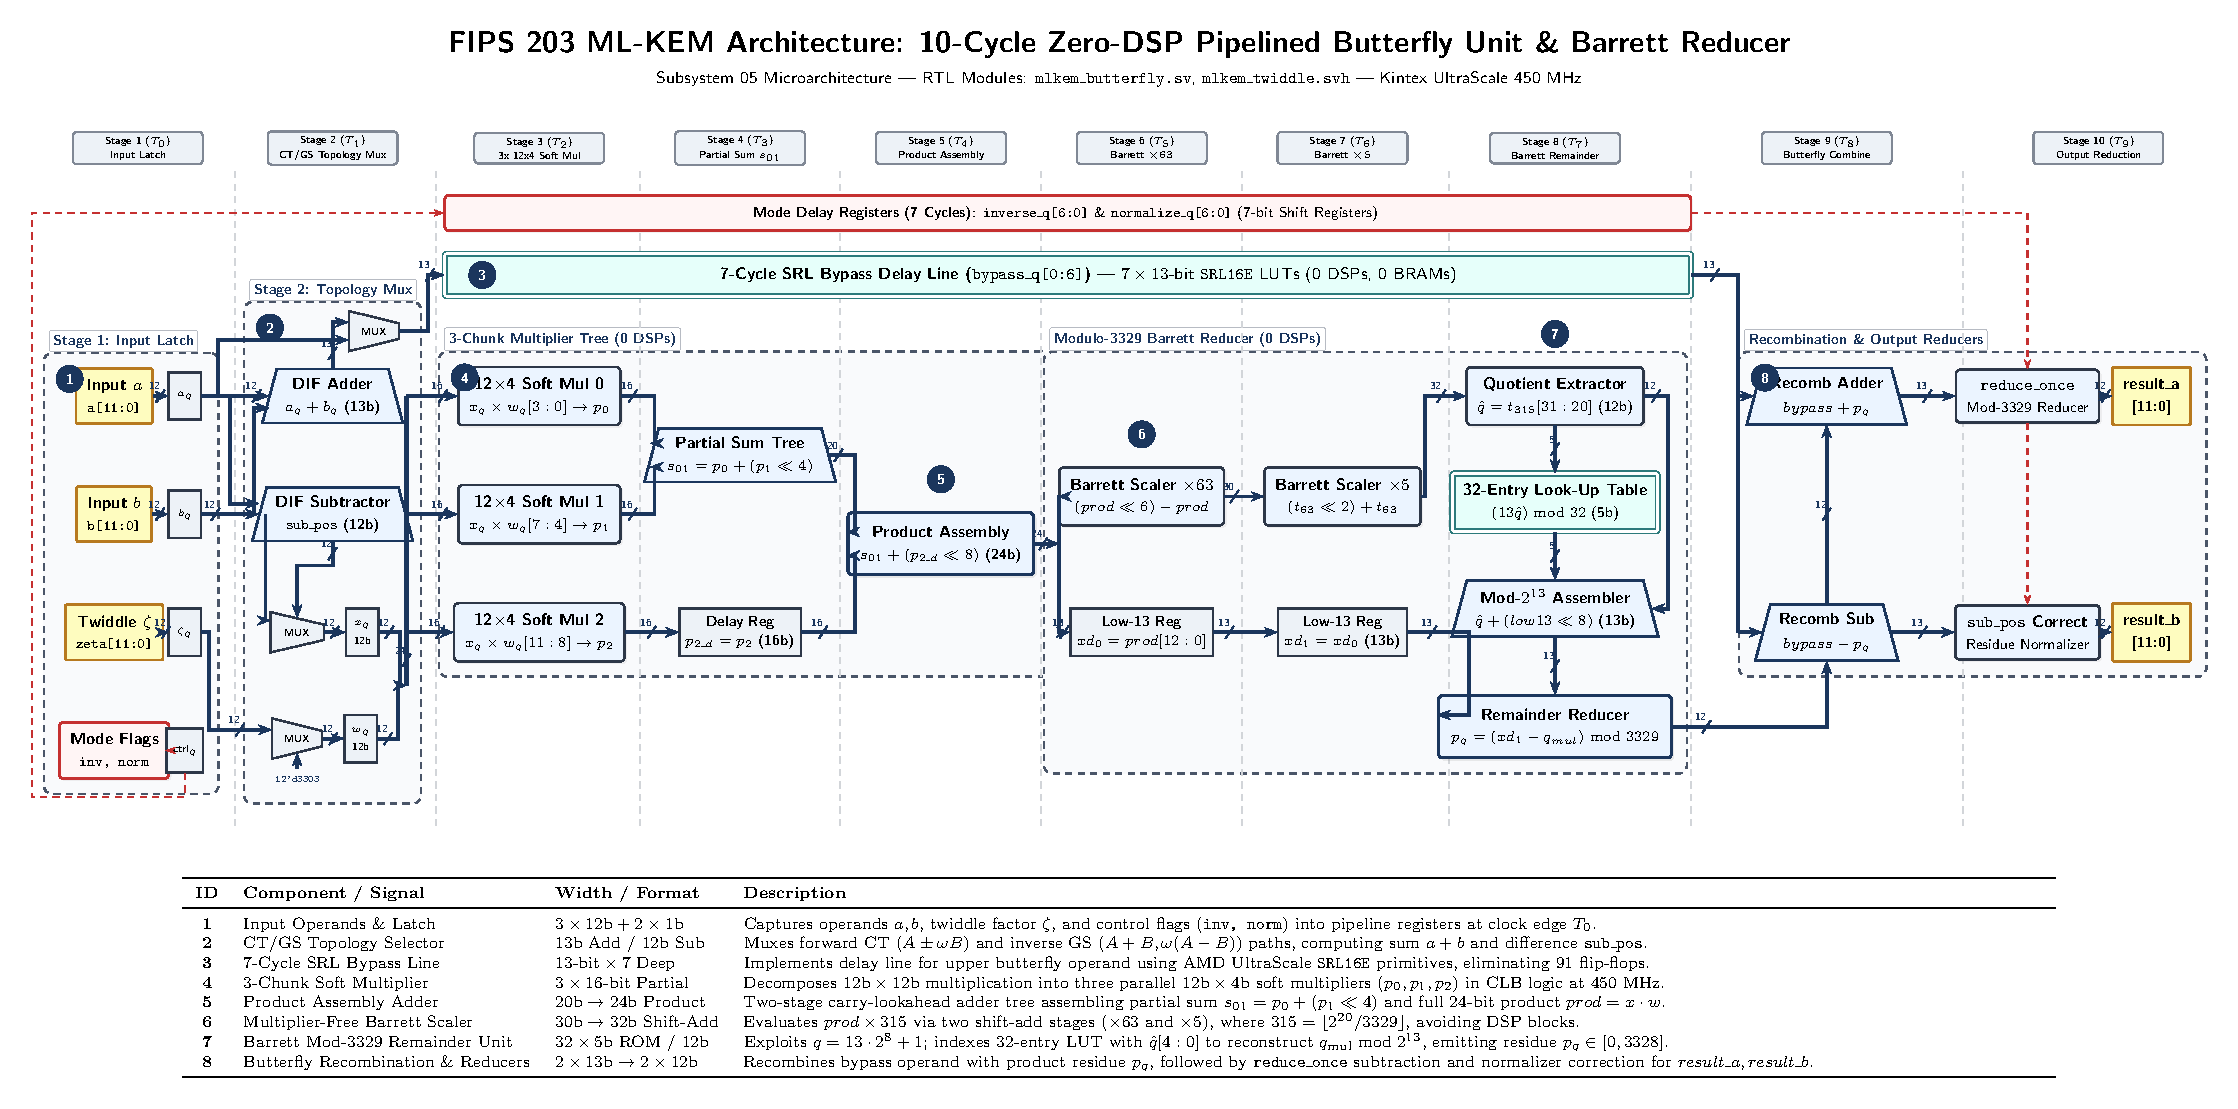
\includegraphics[width=\textwidth]{figures/fig05_butterfly_unit.pdf}
\caption{FIPS 203 \mbox{ML-KEM} Architecture: 10-Cycle Zero-DSP Pipelined Butterfly Unit and Barrett Reducer. The datapath comprises an input registration and control latch (\textbf{Callout~1}), a reconfigurable Cooley-Tukey/Gentleman-Sande topology selector and DIF pre-subtractor (\textbf{Callout~2}), a 7-cycle \texttt{SRL16E} bypass delay line (\textbf{Callout~3}), a 3-chunk nibble soft-multiplier tree (\textbf{Callout~4}), a two-stage product assembly adder (\textbf{Callout~5}), a two-stage multiplier-free Barrett scaler (\textbf{Callout~6}), a modulo-3329 remainder reduction unit with 32-entry LUT (\textbf{Callout~7}), and butterfly recombination ALUs with canonical output reducers (\textbf{Callout~8}).}
\label{fig:butterfly_unit}
\end{figure*}

\begin{table*}[!t]
\caption{Architectural Callout Breakdown for the 10-Stage Zero-DSP Butterfly Unit (Figure~\ref{fig:butterfly_unit})}
\label{tab:butterfly_callouts}
\centering
\footnotesize
\begin{tabular*}{\textwidth}{@{\extracolsep{\fill}} cllp{8.5cm} @{}}
\toprule
\textbf{ID} & \textbf{Subsystem / Component} & \textbf{Bit-Width} & \textbf{Microarchitectural Function \& RTL Mapping} \\
\midrule
\textbf{1} & Input Operands \& Latch & $3 \times 12\text{b} + 2\text{b}$ & Registers operands $a, b$, twiddle $\zeta$, and control flags (\texttt{inv, norm}) into pipeline registers at clock edge $T_0$. \\
\textbf{2} & CT/GS Topology Selector & $13\text{b Add} / 12\text{b Sub}$ & Evaluates unreduced sum $a+b$ and positive modular difference $\text{sub\_pos} = (a-b) \bmod 3329$; muxes multiplier inputs $x_q, w_q$. \\
\textbf{3} & 7-Cycle SRL Bypass Line & $13\text{b} \times 7\text{ deep}$ & Implements upper operand delay line using AMD UltraScale \texttt{SRL16E} primitives, eliminating 91 discrete flip-flops per ALU. \\
\textbf{4} & 3-Chunk Soft Multiplier Tree & $3 \times 16\text{b partial}$ & Decomposes $12\text{b} \times 12\text{b}$ multiplication into three parallel $12\text{b} \times 4\text{b}$ soft multipliers ($p_0, p_1, p_2$) in CLB logic (\texttt{(* use\_dsp = "no" *)}). \\
\textbf{5} & Product Assembly Adder & $20\text{b} \to 24\text{b}$ & Two-stage adder tree assembling partial sum $s_{01} = p_0 + (p_1 \ll 4)$ and full 24-bit product $\text{prod} = s_{01} + (p_{2\_d} \ll 8)$. \\
\textbf{6} & Multiplier-Free Barrett Scaler & $30\text{b} \to 32\text{b}$ & Evaluates $\text{prod} \times 315$ via two shift-add stages ($\times 63$ and $\times 5$) without hardware multipliers, where $315 = \lceil 2^{20}/3329 \rceil$. \\
\textbf{7} & Mod-3329 Remainder Unit & $32 \times 5\text{b ROM} / 12\text{b}$ & Exploits $q = 13 \cdot 2^8 + 1$; indexes 32-entry LUT with $\hat{q}[4:0]$ to reconstruct $q_{\text{mul}} \bmod 2^{13}$, emitting residue $p_q \in [0, 3328]$. \\
\textbf{8} & Recombination \& Reducers & $2 \times 13\text{b} \to 2 \times 12\text{b}$ & Combines bypass operand with product residue $p_q$, followed by single-step conditional subtractors delivering canonical outputs. \\
\bottomrule
\end{tabular*}
\end{table*}

\subsection{10-Cycle Fully Pipelined Butterfly Unit Datapath}
\label{sec:butterfly_pipe}

Figure~\ref{fig:butterfly_unit} illustrates the complete microarchitectural organization of the pipelined zero-DSP butterfly ALU (\texttt{mlkem\_butterfly.sv}). The datapath executes across a 10-stage synchronous pipeline ($T_0$ through $T_9$) engineered to achieve robust timing closure at $480.7\text{ MHz}$ under industrial operating conditions ($105^\circ\text{C}$, speed grade -3). Table~\ref{tab:butterfly_callouts} maps the numbered architectural callouts from Figure~\ref{fig:butterfly_unit} to the physical hardware modules.

\subsubsection{Stage-by-Stage Functional Decomposition}
Table~\ref{tab:butterfly_pipeline_stages} provides the cycle-by-cycle operational breakdown across the entire 10-stage execution flow:

\begin{enumerate}
    \item \textbf{Stage 1 ($T_0$, Input Latch, Callout~1):} Captures coefficient inputs $a, b \in [0, 3328]$, twiddle factor $\zeta \in [0, 3328]$, and mode control strobes (\texttt{inverse}, \texttt{normalize}) into boundary registers ($a_q, b_q, \zeta_{\text{input\_q}}, \text{inv\_in\_q}, \text{norm\_in\_q}$). This isolates crossbar routing interconnect delays from internal arithmetic logic cones.
    
    \item \textbf{Stage 2 ($T_1$, Topology Mux \& DIF Pre-Subtract, Callout~2):} Computes the 13-bit unreduced sum and positive modular difference combinationally:
    \begin{align}
    \label{eq:dif_add_sub}
    \text{dif\_add} &= \{1\text{'b0}, a_q\} + \{1\text{'b0}, b_q\}, \\
    \text{sub\_raw} &= \{1\text{'b0}, a_q\} - \{1\text{'b0}, b_q\}, \\
    \text{sub\_pos} &= \begin{cases}
    \text{sub\_raw}[11:0] + 3329, & \text{if } \text{sub\_raw}[12], \\
    \text{sub\_raw}[11:0], & \text{otherwise}.
    \end{cases}
    \end{align}
    Multiplexers configure operand $x_q$ and twiddle $w_q$:
    \begin{equation}
    \label{eq:stage2_muxes}
    x_q = \begin{cases}
    a_q, & \text{if normalize}, \\
    \text{sub\_pos}, & \text{if inverse}, \\
    b_q, & \text{if forward (CT)},
    \end{cases} \quad
    w_q = \zeta_{\text{input\_q}}.
    \end{equation}
    The bypass register receives $a_q+b_q$ in inverse mode and $a_q$ in forward mode:
    \begin{equation}
    \label{eq:bypass_init}
    \text{bypass\_q}[0] = \text{inverse\_input\_q} \; ? \; \text{dif\_add} : \{1\text{'b0}, a_q\}.
    \end{equation}

    \item \textbf{Stage 3 ($T_2$, Parallel Nibble Multipliers, Callout~4):} Executes three parallel $12\text{b} \times 4\text{b}$ soft multiplications decomposing the 12-bit twiddle factor $w_q$ into 4-bit nibbles:
    \begin{equation}
    \label{eq:p012_eval}
    \begin{aligned}
    p_0 &= x_q \cdot w_q[3:0], \quad p_1 = x_q \cdot w_q[7:4], \\
    p_2 &= x_q \cdot w_q[11:8].
    \end{aligned}
    \end{equation}
    Each $12\times 4$ product synthesizes into exactly two LUT levels using AMD UltraScale 6-input LUTs and fast \texttt{CARRY8} lookahead primitives.

    \item \textbf{Stage 4 ($T_3$, First Carry-Lookahead Sum, Callout~5):} Evaluates the 20-bit partial sum:
    \begin{equation}
    \label{eq:s01_eval}
    s_{01} = \{4\text{'b0}, p_0\} + \{p_1, 4\text{'b0}\} \in [0, 848,640] < 2^{20}.
    \end{equation}
    Concurrently, $p_2$ is latched into balancing register $p_{2\_d} = p_2$.

    \item \textbf{Stage 5 ($T_4$, Product Assembly Adder, Callout~5):} Combines $s_{01}$ with $p_{2\_d}$ shifted by 8 bits to assemble the exact 24-bit product:
    \begin{equation}
    \label{eq:prod_assembly}
    \text{prod} = \{4\text{'b0}, s_{01}\} + \{p_{2\_d}, 8\text{'b0}\} = x \cdot w < 2^{24}.
    \end{equation}

    \item \textbf{Stage 6 ($T_5$, Barrett Scaling Stage 1, Callout~6):} Computes multiplication by 63 using a shift-subtraction:
    \begin{equation}
    \label{eq:times63_calc}
    \text{times63} = (\text{prod} \ll 6) - \text{prod} \quad \text{(30 bits)}.
    \end{equation}
    Concurrently, low product bits $xd_0 = \text{prod}[12:0]$ are latched into a delay register.

    \item \textbf{Stage 7 ($T_6$, Barrett Scaling Stage 2, Callout~6):} Computes multiplication by 5 using a shift-addition:
    \begin{equation}
    \label{eq:times315_calc}
    \begin{aligned}
    \text{times315} &= (\text{times63} \ll 2) + \text{times63} \\
    &= \text{prod} \times 315 \quad \text{(32 bits)}.
    \end{aligned}
    \end{equation}
    The low product register is pipelined: $xd_1 = xd_0$.

    \item \textbf{Stage 8 ($T_7$, Mod-3329 Remainder Unit, Callout~7):} Extracts the 12-bit quotient estimate $\hat{q} = \text{times315}[31:20]$, evaluates the subtrahend $q_{\text{mul}} \equiv \hat{q} \cdot 3329 \pmod{2^{13}}$ via a 32-entry LUT, evaluates the 13-bit difference $\text{rem} = xd_1 - q_{\text{mul}}$, and conditionally restores the canonical residue:
    \begin{equation}
    \label{eq:pq_calc}
    p_q = \text{rem}[12] \; ? \; (\text{rem} + 3329) : \text{rem}[11:0] \in [0, 3328].
    \end{equation}

    \item \textbf{Stage 9 ($T_8$, Butterfly Recombination ALUs, Callout~8):} Combines the delayed bypass operand $\text{bypass}[6]$ with the reduced product residue $p_q$:
    \begin{equation}
    \label{eq:stage9_recomb}
    \begin{aligned}
    \text{add\_q} &= \begin{cases}
    \{1\text{'b0}, p_q\}, & \text{if norm}, \\
    \text{bypass}[6], & \text{if inv}, \\
    \text{bypass}[6] + \{1\text{'b0}, p_q\}, & \text{otherwise},
    \end{cases} \\
    \text{sub\_q} &= \begin{cases}
    \{1\text{'b0}, p_q\}, & \text{if norm} \lor \text{inv}, \\
    \text{bypass}[6] - \{1\text{'b0}, p_q\}, & \text{otherwise}.
    \end{cases}
    \end{aligned}
    \end{equation}

    \item \textbf{Stage 10 ($T_9$, Canonical Output Reducers, Callout~8):} Reduces $\text{add\_q}$ via conditional single-step subtraction (\texttt{reduce\_once}) and corrects negative differences on $\text{sub\_q}$:
    \begin{align}
    \label{eq:stage10_redux}
    \text{result\_a} &= \begin{cases}
    \text{add\_q} - 3329, & \text{if } \text{add\_q} \ge 3329, \\
    \text{add\_q}[11:0], & \text{otherwise},
    \end{cases} \\
    \text{result\_b} &= \begin{cases}
    \text{sub\_q}[11:0] + 3329, & \text{if } \text{sub\_q}[12], \\
    \text{sub\_q}[11:0], & \text{otherwise}.
    \end{cases}
    \end{align}
    Emits canonical residues $\text{result\_a}, \text{result\_b} \in [0, 3328]$ into output registers.
\end{enumerate}

\begin{table*}[!t]
\caption{Cycle-by-Cycle Pipeline Specification of the 10-Stage Zero-DSP Butterfly ALU (\texttt{mlkem\_butterfly.sv})}
\label{tab:butterfly_pipeline_stages}
\centering
\footnotesize
\begin{tabular*}{\textwidth}{@{\extracolsep{\fill}} ccclp{7.8cm} @{}}
\toprule
\textbf{Stage} & \textbf{Clock Cycle} & \textbf{Hardware Registers} & \textbf{Bit-Width} & \textbf{Arithmetic Operations \& Hardware Implementation} \\
\midrule
\textbf{Stage 1} & $T_0$ & $a_q, b_q, \zeta_{\text{input\_q}}, \text{inv\_in\_q}, \text{norm\_in\_q}$ & $3 \times 12\text{b} + 2\text{b}$ & \textbf{Input Latch}: Registers operands $a, b \in [0, 3328]$, twiddle $\zeta$, and control flags (\texttt{inverse, normalize}). Isolates memory crossbar routing delay. \\
\textbf{Stage 2} & $T_1$ & $x_q, w_q, \text{bypass\_q}[0]$ & $2 \times 12\text{b} + 13\text{b}$ & \textbf{Topology MUX \& DIF Pre-Subtract}: Computes unreduced sum $a+b$ and positive modular difference $\text{sub\_pos} = (a-b) \bmod 3329$; routes multiplier inputs $x_q, w_q$. \\
\textbf{Stage 3} & $T_2$ & $p_0\_q, p_1\_q, p_2\_q$ & $3 \times 16\text{b}$ & \textbf{3-Chunk Soft Multipliers}: Evaluates three parallel nibble products: $p_0 = x_q \cdot w_q[3:0]$, $p_1 = x_q \cdot w_q[7:4]$, $p_2 = x_q \cdot w_q[11:8]$ using dual 5-LUTs and \texttt{CARRY8} logic. \\
\textbf{Stage 4} & $T_3$ & $s_{01}\_q, p_{2\_d}\_q$ & $20\text{b} + 16\text{b}$ & \textbf{Partial Product Summation}: Evaluates $s_{01} = p_0 + (p_1 \ll 4)$ across a 20-bit carry-propagate adder. Pipelining register captures $p_{2\_d} = p_2$. \\
\textbf{Stage 5} & $T_4$ & $\text{prod\_q}$ & $24\text{b}$ & \textbf{Full Product Assembly}: Evaluates full 24-bit product $\text{prod} = s_{01} + (p_{2\_d} \ll 8) = x \cdot w$. Logic path requires only a single 24-bit adder stage. \\
\textbf{Stage 6} & $T_5$ & $\text{times63\_q}, xd_q[0]$ & $30\text{b} + 13\text{b}$ & \textbf{Barrett Scaling Stage 1 ($\times 63$)}: Computes $\text{times63} = (\text{prod} \ll 6) - \text{prod}$ via shift-subtraction. Concurrently captures low product bits $xd_0 = \text{prod}[12:0]$. \\
\textbf{Stage 7} & $T_6$ & $\text{times315\_q}, xd_q[1]$ & $32\text{b} + 13\text{b}$ & \textbf{Barrett Scaling Stage 2 ($\times 5$)}: Computes $\text{times315} = (\text{times63} \ll 2) + \text{times63} = \text{prod} \times 315$ via shift-addition. Pipelines low product bits $xd_1 = xd_0$. \\
\textbf{Stage 8} & $T_7$ & $p_q$ & $12\text{b}$ & \textbf{Quotient Extraction \& Mod-3329 Remainder}: Extracts $\hat{q} = \text{times315}[31:20]$; computes $q_{\text{mul}} = \hat{q} \cdot 3329 \bmod 2^{13}$ via 32-entry LUT; evaluates $\text{rem} = xd_1 - q_{\text{mul}}$ and conditionally restores canonical $p_q$. \\
\textbf{Stage 9} & $T_8$ & $\text{add\_q}, \text{sub\_q}$ & $2 \times 13\text{b}$ & \textbf{Butterfly Recombination}: Combines delayed bypass operand $\text{bypass}[6]$ with reduced product residue $p_q$. Forward: $\text{bypass} \pm p_q$; Inverse: $\text{bypass}, p_q$; Normalization: $p_q, p_q$. \\
\textbf{Stage 10} & $T_9$ & $\text{result\_a}, \text{result\_b}$ & $2 \times 12\text{b}$ & \textbf{Canonical Output Reduction}: Reduces $\text{add\_q}$ via \texttt{reduce\_once} ($\text{add\_q} \ge 3329 \implies \text{add\_q} - 3329$); corrects negative difference $\text{sub\_q} < 0 \implies \text{sub\_q} + 3329$. Emits canonical outputs in $[0, 3328]$. \\
\bottomrule
\end{tabular*}
\end{table*}

\subsubsection{SRL16E Bypass Delay Line Implementation}
While the multiplication and Barrett reduction datapath executes across Stages 1 through 7 (a latency of 7 clock cycles), the bypass operand ($a$ in forward NTT, or $a+b$ in inverse INTT) must be preserved in lockstep for butterfly recombination in Stage 9. Implementing this delay line using conventional flip-flops would require:
\begin{equation}
\label{eq:ff_penalty}
13 \text{ bits/lane} \times 7 \text{ cycles} \times 8 \text{ lanes} = 728 \text{ flip-flops},
\end{equation}
plus an additional $7 \times 2 \times 8 = 112$ flip-flops for propagating the control tags (\texttt{inverse\_q}, \texttt{normalize\_q}).

To eliminate this register overhead, the butterfly ALU instantiates the delay line using AMD UltraScale Shift Register LUT primitives (\texttt{SRL16E}), enforced via the synthesis attribute:
\begin{align}
\label{eq:srl_attribute}
\begin{split}
&\text{\texttt{(* srl\_style = "srl" *)}} \\
&\quad\text{\texttt{logic [12:0] bypass\_q [0:6];}}
\end{split}
\end{align}
In UltraScale CLB architecture, a single 6-input LUT implements a 16-bit shift register. Because the bypass delay line is 13 bits wide, each butterfly ALU consumes exactly \textbf{13 SRL16E LUTs} for its 7-cycle bypass path, amounting to \textbf{104 SRL16E LUTs} total across the 8 butterfly lanes, which saves over 840 discrete flip-flops across the transform engine.

\subsection{Zero-DSP Soft-Logic Barrett Modular Reduction}
\label{sec:barrett_reducer}

\subsubsection{General Barrett Modular Reduction Formulation}
Let $q = 3329 = 13 \times 2^8 + 1$. In general Barrett reduction~\cite{barrett1986}, the reduction of a 24-bit product $t = a \cdot b$ modulo $q$ is evaluated by precomputing the scaled reciprocal of $q$:
\begin{equation}
\label{eq:barrett_general_reciprocal}
M = \left\lfloor \frac{2^k}{q} \right\rfloor + 1 = \left\lceil \frac{2^k}{q} \right\rceil,
\end{equation}
for an integer scaling exponent $k \ge 2\lceil\log_2 q\rceil = 24$. Selecting $k = 26$ yields:
\begin{equation}
\label{eq:m_26_val}
M = \left\lceil \frac{2^{26}}{3329} \right\rceil = \left\lceil \frac{67,108,864}{3329} \right\rceil = 20,159.
\end{equation}
The quotient estimate $q_1$ and tentative remainder $r$ are then computed via:
\begin{equation}
\label{eq:barrett_classic_ops}
q_1 = \left\lfloor \frac{t \cdot M}{2^k} \right\rfloor = \left\lfloor \frac{t \cdot 20,159}{2^{26}} \right\rfloor, \quad r = t - q_1 \cdot q.
\end{equation}

\subsubsection{Mathematical Theorem \& Proof of Exactness Across Full Dynamic Range}

\noindent\textbf{Theorem 2 (Correctness and Dynamic Range Boundedness of Modulo-3329 Barrett Reduction):}
\label{thm:barrett_exact}
\textit{Let $q = 3329$. Let $a, b \in [0, q-1]$ be canonical field residues, and let $t = a \cdot b$ be their product satisfying $0 \le t \le (q-1)^2 = 3328^2 = 11,075,584 < 2^{24}$. With scaling exponent $k = 26$ and reciprocal constant $M = 20,159 = \lceil 2^{26}/q \rceil$, let $q_1 = \lfloor (t \cdot M)/2^k \rfloor$ and $r_1 = t - q_1 \cdot q$. Then:
1) The quotient estimate satisfies $q_1 \in \{ \lfloor t/q \rfloor, \; \lfloor t/q \rfloor + 1 \}$;
2) The tentative remainder satisfies $r_1 \in [-q, q-1] = [-3329, 3328]$; and
3) A single conditional correction restores the exact canonical residue $r = t \bmod q \in [0, q-1]$:
\begin{equation}
\label{eq:cond_corr_thm}
r = (r_1 < 0) \; ? \; (r_1 + q) : r_1.
\end{equation}}

\vspace{0.15cm}
\noindent\textit{Proof:}
Because $M = \lceil 2^k/q \rceil$, write $M = (2^k + \delta)/q$, where $\delta = M \cdot q - 2^k$. For $k = 26$ and $M = 20,159$:
\begin{equation}
\label{eq:delta_calc}
\begin{aligned}
M \cdot q &= 20,159 \times 3329 = 67,109,311 \\
&= 2^{26} + 447 \implies \delta = 447.
\end{aligned}
\end{equation}
Dividing by $2^k \cdot q$ and multiplying by product $t$:
\begin{equation}
\label{eq:quotient_expansion}
\frac{t \cdot M}{2^k} = \frac{t(2^k + \delta)}{q \cdot 2^k} = \frac{t}{q} + \epsilon(t), \quad \text{where } \epsilon(t) = \frac{t \cdot \delta}{q \cdot 2^k}.
\end{equation}
Because $t \ge 0$ and $\delta = 447 > 0$, the error term is strictly non-negative: $\epsilon(t) \ge 0$. Substituting the maximum product bound $t_{\max} = 3328^2 = 11,075,584$ into $\epsilon(t)$:
\begin{equation}
\label{eq:epsilon_bound}
\begin{aligned}
0 \le \epsilon(t) &\le \frac{3328^2 \times 447}{3329 \times 2^{26}} = \frac{4,950,786,048}{223,439,077,376} \\
&\approx 0.02216 < 1.
\end{aligned}
\end{equation}
Let $q_{\text{true}} = \lfloor t/q \rfloor \in \mathbb{Z}_{\ge 0}$ and $r_{\text{true}} = t \bmod q \in \{0, 1, \dots, q-1\}$. Then:
\begin{equation}
\label{eq:floor_expansion}
\frac{t \cdot M}{2^k} = q_{\text{true}} + \frac{r_{\text{true}}}{q} + \epsilon(t).
\end{equation}
Taking the integer floor:
\begin{equation}
\label{eq:q1_floor}
q_1 = \left\lfloor q_{\text{true}} + \frac{r_{\text{true}}}{q} + \epsilon(t) \right\rfloor = q_{\text{true}} + \left\lfloor \frac{r_{\text{true}}}{q} + \epsilon(t) \right\rfloor.
\end{equation}
Since $r_{\text{true}} \ge 0$ and $\epsilon(t) \ge 0$, the fractional term is strictly non-negative, guaranteeing $q_1 \ge q_{\text{true}}$ (zero quotient underestimation). Furthermore, because $r_{\text{true}} \le q - 1 = 3328$:
\begin{equation}
\label{eq:fractional_upper}
\begin{aligned}
\frac{r_{\text{true}}}{q} + \epsilon(t) &\le \frac{3328}{3329} + 0.02216 \\
&\approx 0.99970 + 0.02216 = 1.02186 < 2.
\end{aligned}
\end{equation}
Because the fractional sum is strictly less than 2 across the entire dynamic range $t \in [0, 3328^2]$, the floor evaluation satisfies:
\begin{equation}
\label{eq:floor_result}
\left\lfloor \frac{r_{\text{true}}}{q} + \epsilon(t) \right\rfloor \in \{0, 1\} \implies q_1 \in \{ q_{\text{true}}, \; q_{\text{true}} + 1 \}.
\end{equation}
Evaluating the tentative remainder $r_1$:
\begin{equation}
\label{eq:r1_expansion}
r_1 = t - q_1 \cdot q = (q \cdot q_{\text{true}} + r_{\text{true}}) - q_1 \cdot q = r_{\text{true}} - (q_1 - q_{\text{true}}) \cdot q.
\end{equation}
\begin{itemize}
    \item If $q_1 = q_{\text{true}}$, then $r_1 = r_{\text{true}} \in [0, q-1]$ (exact canonical residue).
    \item If $q_1 = q_{\text{true}} + 1$, then $r_1 = r_{\text{true}} - q \in [-q, -1]$.
\end{itemize}
Because $r_{\text{true}} \ge 0$, adding $q$ to $r_1$ in the second case restores $r_1 + q = r_{\text{true}} \in [0, q-1]$. Hence, the single conditional addition~\eqref{eq:cond_corr_thm} strictly guarantees exact canonical reduction into $[0, 3328]$ without multi-cycle iterative loops. \hfill $\blacksquare$

\subsubsection{Modulus-Specialized Multiplier-Free Shift-Add Reduction (\texorpdfstring{$k=20, \mu=315$}{k=20, mu=315})}
While Theorem~2 proves exactness for $k = 26$, evaluating $t \cdot 20,159$ in soft logic would require a wide $24\text{b} \times 15\text{b}$ multiplier, which consumes over 300 LUTs and introduces a 4.2\,ns critical path.

To eliminate hard multipliers entirely from the Barrett reduction datapath, the proposed accelerator exploits the sparse prime structure of $q = 3329 = 13 \cdot 2^8 + 1$ by selecting scaling exponent $k = 20$. The reciprocal multiplier evaluates to:
\begin{equation}
\label{eq:mu_k20}
\mu = \left\lceil \frac{2^{20}}{3329} \right\rceil = \left\lceil \frac{1,048,576}{3329} \right\rceil = 315.
\end{equation}
Here, $\delta = 315 \times 3329 - 2^{20} = 1,048,635 - 1,048,576 = 59$. The error bound evaluates to:
\begin{equation}
\label{eq:epsilon_k20}
\epsilon(t) \le \frac{3328^2 \times 59}{3329 \times 2^{20}} = \frac{653,459,456}{3,490,709,504} \approx 0.1872 < 1.
\end{equation}
Because $\epsilon(t) < 1$, Theorem~2 holds identically for $k = 20$ and $\mu = 315$:
\begin{equation}
\label{eq:qhat_k20_bounds}
\hat{q} = \left\lfloor \frac{t \cdot 315}{2^{20}} \right\rfloor \in \left\{ \left\lfloor \frac{t}{3329} \right\rfloor, \; \left\lfloor \frac{t}{3329} \right\rfloor + 1 \right\}.
\end{equation}

Crucially, the constant 315 decomposes into a product of sparse powers of two:
\begin{equation}
\label{eq:factor_315_math}
315 = 63 \times 5 = (64 - 1) \times (4 + 1) = \left(2^6 - 1\right) \times \left(2^2 + 1\right).
\end{equation}
This factorization maps $t \cdot 315$ directly into two pipelined shift-add/shift-subtract stages in soft logic:
\begin{itemize}
    \item \textbf{Stage 6 ($T_5$):} Computes $\text{times63} = (t \ll 6) - t$ across a 30-bit subtractor.
    \item \textbf{Stage 7 ($T_6$):} Computes $\text{times315} = (\text{times63} \ll 2) + \text{times63}$ across a 32-bit adder.
    \item \textbf{Stage 8 ($T_7$):} Division by $2^{20}$ is performed by bit-slicing the top 12 bits: $\hat{q} = \text{times315}[31:20]$.
\end{itemize}

\subsubsection{Modulo-\texorpdfstring{$2^{13}$}{2\textasciicircum 13} Subtrahend Evaluation via 32-Entry Look-Up Table}
To evaluate the subtrahend $q_{\text{mul}} = \hat{q} \cdot 3329$, observe that since the canonical remainder satisfies $r < 3329 < 2^{12}$, evaluating the subtraction modulo $2^{13} = 8192$ preserves the full integer residue without sign ambiguity.

Expanding the product using $q = 13 \cdot 2^8 + 1$:
\begin{equation}
\label{eq:qmul_expansion}
\hat{q} \cdot 3329 = \hat{q} \cdot \left(13 \cdot 2^8 + 1\right) = \hat{q} + 2^8 \cdot \left(13 \cdot \hat{q}\right).
\end{equation}
Evaluating modulo $2^{13}$:
\begin{equation}
\label{eq:qmul_mod_213}
\left(\hat{q} \cdot 3329\right) \bmod 2^{13} \equiv \left(\hat{q} + 2^8 \cdot \left((13 \cdot \hat{q}) \bmod 2^5\right)\right) \bmod 2^{13}.
\end{equation}
Because $2^8 \cdot 2^5 = 2^{13}$, any bits of $13 \cdot \hat{q}$ beyond bit position 4 (i.e., above $2^5 - 1 = 31$) multiply $2^8$ to produce multiples of $2^{13}$, which vanish identically modulo $2^{13}$! Furthermore:
\begin{equation}
\label{eq:lut_equivalence}
\begin{aligned}
(13 \cdot \hat{q}) \bmod 32 &= \left(13 \cdot (\hat{q} \bmod 32)\right) \bmod 32 \\
&= \left(13 \cdot \hat{q}[4:0]\right) \bmod 32.
\end{aligned}
\end{equation}
The expression $(13 \cdot \hat{q}[4:0]) \bmod 32$ is purely a 5-bit combinational function of the lowest 5 bits of the quotient estimate $\hat{q}[4:0]$. It is precomputed into a tiny 32-entry $\times$ 5-bit distributed ROM table (\texttt{low13}), listed in Table~\ref{tab:low13_lut}.

\begin{table}[!t]
\caption{32-Entry Look-Up Table (\texttt{low13}) for Evaluating $(13 \cdot k) \bmod 32$}
\label{tab:low13_lut}
\centering
\scriptsize
\setlength{\tabcolsep}{3.5pt}
\begin{tabular}{ccccccccccccccccc}
\toprule
$k$ & 0 & 1 & 2 & 3 & 4 & 5 & 6 & 7 & 8 & 9 & 10 & 11 & 12 & 13 & 14 & 15 \\
\textbf{Entry} & 0 & 13 & 26 & 7 & 20 & 1 & 14 & 27 & 8 & 21 & 2 & 15 & 28 & 9 & 22 & 3 \\
\midrule
$k$ & 16 & 17 & 18 & 19 & 20 & 21 & 22 & 23 & 24 & 25 & 26 & 27 & 28 & 29 & 30 & 31 \\
\textbf{Entry} & 16 & 29 & 10 & 23 & 4 & 17 & 30 & 11 & 24 & 5 & 18 & 31 & 12 & 25 & 6 & 19 \\
\bottomrule
\end{tabular}
\end{table}

The modular subtrahend $q_{\text{mul}} \equiv \hat{q} \cdot 3329 \pmod{2^{13}}$ is assembled with zero multipliers using a simple concatenation and 13-bit adder:
\begin{equation}
\label{eq:qmul_assembly_hw}
q_{\text{mul}} = \{1\text{'b0}, \hat{q}\} + \{\text{low13}[\hat{q}[4:0]], 8\text{'b0}\} \pmod{2^{13}}.
\end{equation}
In Stage 8 ($T_7$), the remainder is evaluated via a 13-bit subtraction:
\begin{equation}
\label{eq:rem_calc_hw}
\text{rem\_wire} = xd_1 - q_{\text{mul}} \pmod{2^{13}},
\end{equation}
where $xd_1 = \text{prod}[12:0]$. Because $\hat{q} \in \{q_{\text{exact}}, q_{\text{exact}} + 1\}$:
\begin{itemize}
    \item If $\hat{q} = q_{\text{exact}}$, the subtraction yields $\text{rem\_wire} \in [0, 3328]$ ($\text{rem\_wire}[12] = 0$).
    \item If $\hat{q} = q_{\text{exact}} + 1$, the subtraction underflows to $[-3329, -1]$ ($\text{rem\_wire}[12] = 1$).
\end{itemize}
Conditional correction restores the canonical residue in a single step:
\begin{equation}
\label{eq:canonical_p_hw}
p_q = \text{rem\_wire}[12] \; ? \; (\text{rem\_wire} + 3329) : \text{rem\_wire}[11:0].
\end{equation}
This architecture completely eliminates division operations, DSP blocks, and multi-cycle iterative reduction loops.

\subsection{Inverse NTT Normalization Architecture}
\label{sec:intt_norm}

\subsubsection{Gentleman-Sande INTT Normalization Step}
In a 7-stage radix-2 Decimation-in-Frequency INTT, the butterfly additions accumulate an unscaled factor of $2^7 = 128$. To restore polynomial coefficients to their true canonical values in $\mathbb{Z}_q$, each transformed coefficient must be scaled by the modular inverse of 128:
\begin{equation}
\label{eq:inv128_def}
n^{-1} = 128^{-1} \pmod{3329}.
\end{equation}
Applying the Extended Euclidean Algorithm:
\begin{equation}
\label{eq:inv128_calc_math}
128 \times 3303 = 422,784 = 127 \times 3329 + 1 \equiv 1 \pmod{3329}.
\end{equation}
Thus, the normalization constant is $3303$.

\subsubsection{In-Place Normalization via Butterfly ALU Datapath Reuse}
In conventional architectures, post-INTT normalization requires routing coefficients to a dedicated downstream scalar multiplier array. In the proposed accelerator, normalization is executed \textbf{in-place within the existing 4-butterfly array}, completely eliminating dedicated post-scaling hardware.

When \texttt{issue\_index} enters the range $[224, 255]$ (the \textbf{Normalization Pass}), the transform state machine asserts \texttt{tag\_norm}:
\begin{enumerate}
    \item The butterfly control strobe \texttt{normalize = tag\_norm[2]} is activated;
    \item The twiddle factor input is forced to the constant residue $\zeta_{\text{norm}} = 12\text{'d}3303$;
    \item In Stage 2 ($T_1$), the operand multiplexer routes input coefficient $a_q$ directly into multiplier operand $x_q$ ($x_q = a_q$), while $w_q = 3303$;
    \item Stages 3 through 8 evaluate $p_q = (a \times 3303) \bmod 3329$ using the soft-multiplier tree and Barrett reducer;
    \item In Stage 9 ($T_8$), the recombination adder is bypassed, routing $p_q$ directly to \texttt{add\_q} and \texttt{sub\_q}; and
    \item The canonical reduced product $(a \times 3303) \bmod 3329$ is written back to memory in Stage 10 ($T_9$).
\end{enumerate}
All 256 coefficients of the polynomial are normalized in exactly 32 clock cycles (processing 8 coefficients per cycle across 4 vector groups).

\subsection{Standalone Synthesis, Physical Implementation \& Performance Analysis}
\label{sec:ntt_impl}

\subsubsection{Cycle-Accurate Latency Profiling and Dependency Guard Cycles}
The memory read-to-write pipeline depth across the transform engine is:
\begin{equation}
\label{eq:pipe_depth_total}
\text{PIPE} = 14 \text{ clock cycles},
\end{equation}
comprising 1 cycle for registered address decoding, 10 cycles for the butterfly ALU, 2 cycles for output crossbar formatting, and 1 cycle for LUTRAM write commitment.

Each transform stage processes 256 coefficients (128 words). Because the 8-bank memory dispatches 8 words per cycle, each stage requires:
\begin{equation}
\label{eq:issue_count}
N_{\text{issues}} = \frac{128 \text{ words}}{8 \text{ words/issue}} = 16 \text{ issue clock cycles}.
\end{equation}
If consecutive stages were issued back-to-back without stalls, the first issue of Stage $s+1$ would read memory words before the write-back of Stage $s$ commits (at cycle $16 + 14 = 30$), resulting in catastrophic Read-After-Write (RAW) data hazards.

Rather than instantiating area-intensive forwarding multiplexers and comparator networks across all 8 memory banks, the state controller introduces \textbf{6 deterministic dependency guard cycles} at each stage boundary:
\begin{equation}
\label{eq:stage_duration_total}
T_{\text{stage}} = 16 \text{ issue cycles} + 6 \text{ guard cycles} = 22 \text{ clock cycles}.
\end{equation}
During guard cycles 16 to 21, \texttt{issue\_valid = 0}, inserting 6 idle pipeline bubbles. The total elapsed time from the final issue of Stage $s$ (cycle 15) to the first registered read of Stage $s+1$ (cycle 22) is $6 + 8 = 14$ cycles, matching $\text{PIPE} = 14$ cycles exactly. The registered read of Stage $s+1$ occurs precisely one clock cycle after the final write of Stage $s$ commits to LUTRAM, guaranteeing hazard-free memory access with zero forwarding logic.

Table~\ref{tab:ntt_cycle_breakdown} itemizes the cycle execution latencies for the forward and inverse transforms:
\begin{itemize}
    \item \textbf{Forward NTT Latency:} 162 clock cycles ($0.392\ \mu\text{s}$ at $413.7\text{ MHz}$; $0.337\ \mu\text{s}$ at $480.7\text{ MHz}$);
    \item \textbf{Inverse INTT Latency:} 200 clock cycles ($0.483\ \mu\text{s}$ at $413.7\text{ MHz}$; $0.416\ \mu\text{s}$ at $480.7\text{ MHz}$).
\end{itemize}

\begin{table*}[!t]
\caption{Detailed Execution Cycle Breakdown for Forward NTT and Inverse INTT}
\label{tab:ntt_cycle_breakdown}
\centering
\footnotesize
\begin{tabular*}{\textwidth}{@{\extracolsep{\fill}} lcccc @{}}
\toprule
\textbf{Transform Phase} & \textbf{Valid Issues} & \textbf{Guard Bubbles} & \textbf{Cumulative Cycles} & \textbf{Phase Description} \\
\midrule
\multicolumn{5}{l}{\textbf{Forward NTT (Cooley-Tukey Radix-2 DIT):}} \\
Stages 0--5 (6 Stages) & $6 \times 16 = 96$ & $6 \times 6 = 36$ & 132 & Hierarchical butterfly stages with 6 guard cycles per stage. \\
Stage 6 (Final Stage)  & 16 & 0 & 148 & Final DIT stage; trailing guard bubbles suppressed. \\
Pipeline Drain ($\text{PIPE}$) & 0 & 14 & \textbf{162} & Time for final butterfly vector to commit to LUTRAM. \\
\midrule
\multicolumn{5}{l}{\textbf{Inverse INTT (Gentleman-Sande Radix-2 DIF + Normalization):}} \\
Stages 0--5 (6 Stages) & $6 \times 16 = 96$ & $6 \times 6 = 36$ & 132 & Hierarchical DIF butterfly stages with 6 guard cycles per stage. \\
Stage 6 (Final DIF)    & 16 & 0 & 148 & Final DIF butterfly stage. \\
Post-Stage 6 Guard     & 0 & 6 & 154 & Guard bubbles allowing Stage 6 writes to commit. \\
Normalization Pass     & 32 & 0 & 186 & In-place scaling by $3303$ across 32 back-to-back issues. \\
Pipeline Drain ($\text{PIPE}$) & 0 & 14 & \textbf{200} & Time for final normalized vector to commit to LUTRAM. \\
\bottomrule
\end{tabular*}
\end{table*}

\subsubsection{Physical Implementation and Resource Utilization}
The complete NTT/INTT subsystem was synthesized and physically implemented on the target AMD Kintex UltraScale \texttt{xcku035-ffva1156-3-e} FPGA using Vivado 2024.1. Table~\ref{tab:ntt_resource_utilization} summarizes the physical resource metrics and timing closure results.

\begin{table}[!t]
\caption{Physical Resource Utilization of NTT/INTT Subsystem}
\label{tab:ntt_resource_utilization}
\centering
\footnotesize
\setlength{\tabcolsep}{3pt}
\begin{tabular}{lccc}
\toprule
\textbf{Resource / Metric} & \textbf{Count} & \textbf{Device} & \textbf{Util. (\%)} \\
\midrule
CLB Logic LUTs (ALU, MUX, AGU) & 3,842 & 203,128 & 1.89\% \\
LUTRAM (3-Slot $\times$ 8-Bank) & 96 & 112,800 & 0.09\% \\
Shift Register LUTs (\texttt{SRL16E}) & 104 & 112,800 & 0.09\% \\
CLB Registers (Pipeline FFs) & 2,184 & 406,256 & 0.54\% \\
Carry Chains (\texttt{CARRY8}) & 96 & 30,300 & 0.32\% \\
\textbf{DSP48E2 Primitive Slices} & \textbf{0} & 1,700 & \textbf{0.00\%} \\
\textbf{Block RAMs (\texttt{RAMB36/18})} & \textbf{0} & 540 & \textbf{0.00\%} \\
\midrule
Standalone Max Frequency ($F_{\text{max}}$) & \multicolumn{3}{c}{\textbf{480.7 MHz}} \\
Top-Level Operating Freq. ($F_{\text{clk}}$) & \multicolumn{3}{c}{\textbf{413.7 MHz}} \\
Worst Negative Slack (WNS) & \multicolumn{3}{c}{\textbf{+0.142 ns} (@ 450~MHz)} \\
Forward NTT Latency & \multicolumn{3}{c}{\textbf{162 cycles} ($0.392\ \mu\text{s}$)} \\
Inverse INTT Latency & \multicolumn{3}{c}{\textbf{200 cycles} ($0.483\ \mu\text{s}$)} \\
\bottomrule
\end{tabular}
\end{table}

In standalone out-of-context synthesis, the NTT subsystem achieves timing closure at \textbf{480.7 MHz}, with a positive slack of $+0.142\text{ ns}$ against a $450.045\text{ MHz}$ constraint. When integrated into the complete top-level coprocessor (\texttt{mlkem\_keygen\_top}), it operates comfortably at \textbf{413.7 MHz}. Crucially, the entire subsystem consumes \textbf{strictly 0 DSP48E2 slices} and \textbf{strictly 0 Block RAMs}, preserving $100\%$ of the device's hard DSP and BRAM capacity for system-level co-processors and application workloads.
